\documentclass[10.5pt, a4, dvipdfmx]{article}

\usepackage{mathedral}
\usepackage{pgf-umlcd}

\title{TITLE}
\author{AUTHOR}
\date{\today}

\newcommand{\attributett}[1]{\attribute{\texttt{#1}}}

\begin{document}
  \maketitle

  \begin{center}
    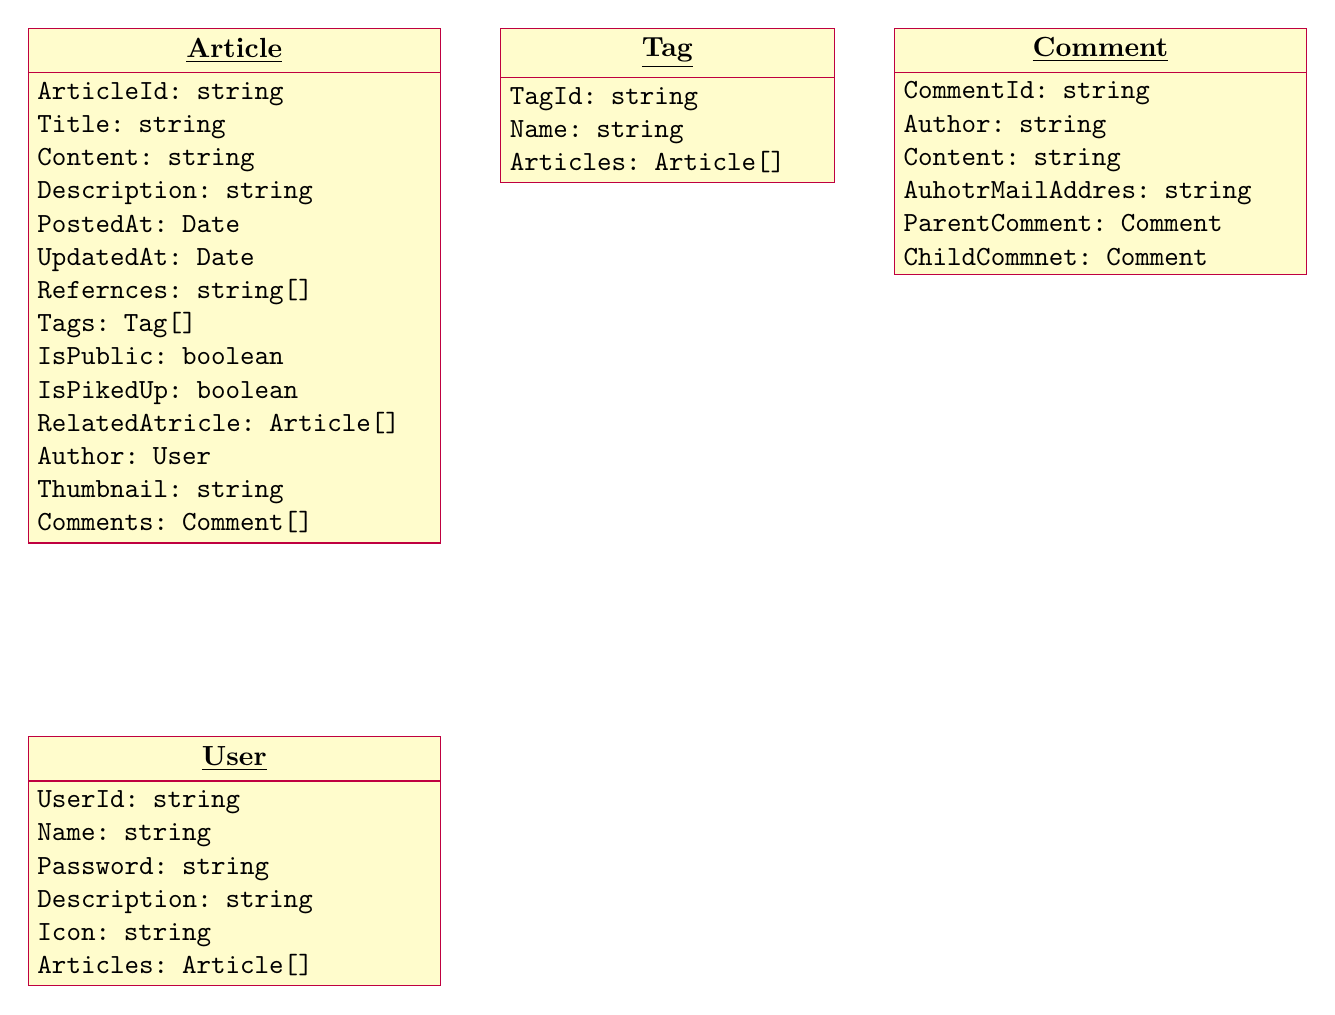
\begin{tikzpicture}
      \begin{object}[text width=5cm]{Article}{0,0}
        \attributett{ArticleId: string}
        \attributett{Title: string}
        \attributett{Content: string}
        \attributett{Description: string}
        \attributett{PostedAt: Date}
        \attributett{UpdatedAt: Date}
        \attributett{Refernces: string[]}
        \attributett{Tags: Tag[]}
        \attributett{IsPublic: boolean}
        \attributett{IsPikedUp: boolean}
        \attributett{RelatedAtricle: Article[]}
        \attributett{Author: User}
        \attributett{Thumbnail: string}
        \attributett{Comments: Comment[]}
      \end{object}
  
      \begin{object}[text width=4cm]{Tag}{5.5,0}
        \attributett{TagId: string}
        \attributett{Name: string}
        \attributett{Articles: Article[]}
      \end{object}
  
      \begin{object}[text width=5cm]{Comment}{11,0}
        \attributett{CommentId: string}
        \attributett{Author: string}
        \attributett{Content: string}
        \attributett{AuhotrMailAddres: string}
        \attributett{ParentComment: Comment}
        \attributett{ChildCommnet: Comment}
      \end{object}

      \begin{object}[text width=5cm]{User}{0,-9}
        \attributett{UserId: string}
        \attributett{Name: string}
        \attributett{Password: string}
        \attributett{Description: string}
        \attributett{Icon: string}
        \attributett{Articles: Article[]}
      \end{object}
    \end{tikzpicture}
  \end{center}
\end{document}